\documentclass{article}
\title{Blockchain Technology SoS Reading Project}

\author{Pagoti Hemanth Naidu - 210050117 \\
Mentor: Shikhar Agrawal}
\date{may 2023}
\usepackage{xcolor}
\usepackage{graphicx}
\usepackage{adjustbox}
\usepackage{titlesec}
\usepackage{listings}
\usepackage{tikz}
\usepackage{amsmath}
\usepackage{hyperref}
\usepackage{tocloft}
\usepackage{tikz}
\usetikzlibrary{automata,positioning}
\usetikzlibrary{positioning}
\usetikzlibrary{shapes,arrows,calc,arrows.meta}
\usepackage{amsmath,bm,times}
\newcommand{\mx}[1]{\mathbf{\bm{#1}}} % Matrix command
\newcommand{\vc}[1]{\mathbf{\bm{#1}}} % Vector command
\renewcommand{\cftsecleader}{\cftdotfill{\cftdotsep}} % Add dots between section title and page number
\begin{document}
\tikzstyle{sensor}=[draw, fill=blue!20, text width=5em, 
text centered, minimum height=2.5em]
\tikzstyle{ann} = [above, text width=6em]
\tikzstyle{naveqs} = [sensor, text width=6em, fill=red!20, 
minimum height=12em, rounded corners]
\def\blockdist{2.3}
\def\edgedist{1}
\maketitle
\tableofcontents
\newpage
\section{Introduction}

Bitcoin was introduced in 2009 by Satoshi Nakamoto in response to the 2008 global financial crisis and the need for a decentralized, peer-to-peer electronic cash system. 
Nakamoto's vision was to create a currency free from central control, censorship-resistant, and capable of secure, borderless transactions.
\subsection{Demand \& Supply of Bitcoin}
Bitcoin's supply is regulated by Satoshi Nakamoto's algorithm, limiting the total number of bitcoins that can ever exist to 21 million.
The demand for bitcoin is determined by market forces and influenced by factors such as investor sentiment and adoption. 
Balancing supply and demand is essential for maintaining stability in the Bitcoin market and mitigating the risk of inflation.
\subsection{Double Spend Problem}
Satoshi Nakamoto's design of Bitcoin ensures that money can only be spent once through the concept of ownership and peer-to-peer networks. With public keys, everyone can know how much each owner possesses while maintaining anonymity. 
Hash functions are used for encoding transactions and mining purposes, while proof of work enables Bitcoin to function as a cryptocurrency. 
The tamper-proof nature of blockchain ensures that once transactions are added, they cannot be modified, and each block in the blockchain contains the hash of the previous block.
Smart contracts are self-executing contracts with the terms of the agreement directly written into code, automating and enforcing the agreed-upon conditions without the need for intermediaries. 
They enable secure and transparent transactions in various applications, from finance to supply chain management.
\section{Motivation}
\subsection{Blockchains in High Level}
\begin{itemize}
    \item Blockchain utilizes a tamperproof data structure that ensures data integrity and security.
    \item Starting with a genesis block, each subsequent block in the chain holds information in the form of bitstrings or binary representations.
    \item Once data is added to a block and appended to the chain, it becomes immutable and cannot be removed or altered.
    \item This feature of blockchain, along with its decentralized and distributed nature enables various applications such as cryptocurrency, smart contracts and trust.
\end{itemize}
\subsection{Applications}
\begin{itemize}
    \item \textbf{Governance}: Land records, health records, transportation data, virtual currency, electronic wills, passport, identification, etc.
    \item \textbf{Commercial}: supply chains, auctions, gaming, sale of music, financial services, smart grid etc.
    \item \textbf{Disruptive}: Cryptocurrencies, Initial Coin Offerings
\end{itemize}
\section{cryptocurrency}
Bitcoin has no central trudtrd authority, cryptography brings in trust and peer to peer networks provide decentralization. Bitcoin satisfies the characteristics of acceptability, portability, durability, divisibility, and fungibility.
\begin{itemize}
\item \textbf{Acceptability}: Bitcoin is widely accepted as a form of payment and store of value.
\item \textbf{Portability}: Bitcoin can be easily transferred and accessed across geographical boundaries.
\item \textbf{Durability}: Bitcoin's digital nature makes it resistant to physical damage or deterioration.
\item \textbf{Divisibility}: Bitcoin is divisible into small units, allowing for precise transactions of any value.
\item \textbf{Fungibility}: Bitcoin units are interchangeable, meaning that each unit holds the same value and can be exchanged without distinction.
\end{itemize}
Each transaction is brodcasted among all so that double spend is avoided. \\
Consensus protocols are mechanisms used in blockchain networks to achieve agreement among participants on the validity of transactions and the order in which they are added to the blockchain and this is also know as proof of work.
\section{Peer to Peer}
A permissionless, distributed system allows an arbitrary number of participants to join or leave at any time, enabling seamless peer-to-peer transactions where individuals have the freedom to pay anyone within the network, fostering inclusivity and decentralization.
\subsection{Consensus Protocol}
\begin{itemize}
\item To establish consensus in a protocol, cryptography is employed to secure transactions and validate the integrity of the data. 
\item While a peer-to-peer network enables direct communication and information sharing among participants. 
\item The proof-of-work mechanism adds a layer of computational effort to validate transactions and prevent malicious behavior, and Merkle trees provide an efficient and verifiable way to store and verify the integrity of large sets of data within the blockchain. 
\item Together, these components form the foundation for a robust and trustless consensus protocol.
\end{itemize}
\subsection{Popular P2P versions}
\subsubsection{Napster}
Napster was one of the earliest peer-to-peer networks that facilitated file sharing. It used a centralized server to maintain an index of available files, allowing users to search and download files directly from each other, enabling widespread file sharing but faced legal challenges due to copyright concerns.
\subsubsection{Gnutella}
Gnutella is a decentralized peer-to-peer network where participating nodes connect directly with each other. It operates on a query flooding mechanism, where search queries propagate across the network, and peers respond with matching files, ensuring a distributed and scalable file sharing system.
\subsubsection{Distributed Hash Table}
DHT is a decentralized peer-to-peer network architecture that provides efficient lookup and storage of key-value pairs. It operates by partitioning the hash space among participating nodes, enabling direct lookup and storage of data based on keys. DHTs provide fault tolerance, scalability, and efficient resource utilization in distributed systems and are commonly used in applications like BitTorrent and distributed storage systems.
\section{Hash functions}
Each block in the blockchain contains hash of the previous block, the hash is recognised as an unique ID.
\subsection{Basic properties of Hash functions}
\begin{itemize}
    \item Input to the hash function can be of any length.
    \item Output of the hash function should be of fixed size.
    \item Hah should be efficiently computed.
\end{itemize}
\subsection{Random Oracle}
It is like a black box that takes input and generates a random output based on that input. It provides a consistent and unpredictable response to any query. Random oracles are often used to model idealized cryptographic functions and serve as a building block for designing secure protocols and systems. \\
However, in practice, real-world hash functions are used as a substitute for random oracles.
\subsection{Properties of Cryptographic Hash functions}
\subsubsection{Collision Resistence}
Collision resistance, in the context of cryptographic hash functions, means that it is computationally infeasible to find two different inputs that produce the same hash output. It ensures that a small change in the input will result in a significantly different hash value, making it difficult to forge or manipulate data without detection. \\
The birthday paradox states that in a group of relatively few people, the probability of two individuals sharing the same birthday is surprisingly high.
\subsubsection{Hiding}
suppose r takes values from $r_1$, $r_2$, $r_3$, ....., $r_n$ with probability  $p(r_1)$, $p(r_2)$, $p(r_3)$, ....., $p(r_n)$. \\
The minimum entropy is defined as follows 
$$min-entropy = min_{i=1}^{n} -log(x_i)$$
where a secret value r is chosen from a probability distribution with high min-entropy and combined with another value x to compute the hash h(x\textbar\textbar r), it is infeasible to find the original value of x given only the hash h(x\textbar\textbar r). \\
\subsubsection{Puzzle Friendliness}
Hash function is puzzle friendly if for every N bit output Y if K is choosen from a probability distribution with high minimum entropy, then it is infeasible to find X such that 
$$H(K||X) = Y$$
in time significantly less than O($2^N$).
\subsection{Proof of Work}
\begin{itemize}
\item Miner selects pending transactions.
\item Miner combines hash of previous block, nonce, and transactions.
\item Nonce is of 16 bits, miner can include any number of transactions.
\item Miner adjusts nonce until the resulting block hash meets the threshold for network consensus, creating the next block.
\item Once a valid block is created it should be brodcasted to other miners for verification.
\end{itemize}
\section{SHA256 and Merkle Trees}
Here's a high-level overview of how SHA-256 works:
\begin{itemize}
\item \textbf{Padding}: The input message is padded with length of message to ensure it meets certain requirements for the SHA-256 algorithm. Padding includes adding bits to the message to make it a multiple of 512 bits.
\item \textbf{Initialization}: An Initialization Vector (IV) is a predetermined set of initial values used to initialize the compression process in certain compression algorithms, ensuring consistent and reproducible compression results for the same input data.
\item \textbf{Processing}: The padded message is divided into blocks of 512 bits, and the algorithm processes each block sequentially. The processing involves a series of logical and bitwise operations, including message expansion, data mixing, and bitwise operations such as AND, OR, and XOR.
\item \textbf{Compression}: Each block is compressed using a combination of logical and bitwise operations, updating the state of the hash values.
\item \textbf{Finalization}: Once all the blocks have been processed, the resulting hash value is obtained by concatenating the updated hash values.
\end{itemize}
Miners use Merkle trees (also known as Merkle hash trees) as an efficient and secure way to summarize a large set of transactions within a blockchain. These trees play a crucial role in the creation of the next block in the blockchain. Let's walk through the process:
\begin{itemize}
    \item Miners gather valid transactions and sort them. They hash each transaction individually and combine the hashed values in pairs until a single root hash, known as the Merkle root, remains at the top of the tree.
    \item The Merkle root is included in the block header along with other block information. Miners attempt to find a nonce value that, when hashed with the block header, produces a hash that is less than the threshold.
\end{itemize}
\subsection{Advantages of Merkle Trees}
\begin{itemize}
    \item Merkle trees enable efficient verification and tamper detection, making it difficult for a miner to modify a specific transaction without changing the Merkle root.
    \item If a miner want to add or Modify a transaction while solving the puzzle it can be done in O(log(M)) operations where M is no of transactions included.
    \item Light clients(New commer of Bitcoin) require fewer resources, enabling users with limited capabilities to participate in blockchain networks.
\end{itemize}
\subsection{Prooving to Light Client}
There is a situation that A is a light clinet and B need to proove that one of his transaction happend to C to A then B can provide A with a compact proof known as a Merkle proof. \\
This proof consists of the transaction, its corresponding Merkle path, and the Merkle root. A can then verify the validity of the transaction by using the Merkle proof to trace the transaction's inclusion in the Merkle tree and comparing the computed Merkle root with the one stored by A.
\subsection{Full Client using Merkle Trees}
If a full client want to discard any of the transaction he stored he can still proove that remaing transactions belonging to the same merkle tree which may not be happend if he stores in a naive way i.e concatenating all the transactions.
\section{Bitcoin Transactions}
\subsection{Block Header contents}
The block header in a blockchain typically contains the following elements:
\begin{itemize}
    \item \textbf{Previous Block Hash}: Hash of the preceding block in the blockchain.
    \item \textbf{Merkle Root}: Hash of all the transactions included in the block.
    \item \textbf{Timestamp}: The time when the block was created, which is used after to find appropriate threshold.
    \item \textbf{Nonce}: A number used in the mining process to find a valid block hash.
    \item \textbf{threshold}: 4 Bytes are used to represnt threshold also known as bits, to save space instead of storing 256 bits.
    $$bits = b_1b_2b_3b_4$$
    $$Threshold = b2_2b_3b_4 * 256^{b_1 - 3}$$
\end{itemize}
\subsection{Digital Signatures}
Digital Signatures are hard to forge, easy to create and easy to verify. \\
These signatures use the below three alogorithms to complete the need:
\subsubsection{Generation of shared, public key pair}
This uses GenerateKeys algorithm which takes key size as the parameter and generates a key pair in which shared key is kept secret and public key is known to everyone.
\subsubsection{sign the message}
This uses Sign algorithm which takes message and shared key as the algorithm and encypts the message, in this case message is typically a transaction. 
\subsubsection{verify the signature}
This uses Verify algorithm which takes the message, signature and cipher text and verify the signature, this is done by everyone to verify transactions.
\subsection{ECDSA}
Elliptic Curve Digital Signature Algorithm is a cryptographic algorithm used for generating and verifying digital signatures, in which public key is 512 bits, shared key is 256 bits, signature is 512 bits and the message should be 256 bits.\\
Hash the message using SHA256 as many of the messages are not of 256 bits.
\subsection{Transactions}
Assume A($SK_A,PK_A$) want to pay B($SK_B,PK_B$),  A has to make a transaction himself and sigh it with his shared key as discussed above. \\
Now the problem is how a miner verify this transaction is valid or not.
\subsubsection{Structure of bitcoin transactions}
\begin{center}
\begin{tikzpicture}[>={Latex[scale=1.5]}]
    %% Encoder
    \node (naveq) [naveqs] {Transaction};
    %% Inputs
    \draw[<-] ($(naveq.south west)!0.9!(naveq.north west)$) -- +(-\edgedist,0) node [left] {$(SK^{i}_0,PK^{i}_0)$};
    \draw[<-] ($(naveq.south west)!0.75!(naveq.north west)$) -- +(-\edgedist,0) node [left] {$(SK^{i}_1,PK^{i}_1)$};
    \draw[<-] ($(naveq.south west)!0.6!(naveq.north west)$) -- +(-\edgedist,0) node [left] {$(SK^{i}_2,PK^{i}_2)$};
    \draw[<-] ($(naveq.south west)!0.45!(naveq.north west)$) -- +(-\edgedist,0) node [left] {$(SK^{i}_3,PK^{i}_3)$};
    \draw[<-] ($(naveq.south west)!0.30!(naveq.north west)$) -- +(-\edgedist,0) node [left] {$(SK^{i}_4,PK^{i}_4)$};
    \draw[<-] ($(naveq.south west)!0.15!(naveq.north west)$) -- +(-\edgedist,0) node [left] {$(SK^{i}_5,PK^{i}_5)$};
    %% Outputs
    \draw[->] ($(naveq.south east)!0.9!(naveq.north east)$) -- +(\edgedist,0) node [right] {$(SK^{o}_0,PK^{o}_0)$};
    \draw[->] ($(naveq.south east)!0.75!(naveq.north east)$) -- +(\edgedist,0) node [right] {$(SK^{o}_1,PK^{o}_1)$};
    \draw[->] ($(naveq.south east)!0.6!(naveq.north east)$) -- +(\edgedist,0) node [right] {$(SK^{o}_2,PK^{o}_2)$};
    \draw[->] ($(naveq.south east)!0.45!(naveq.north east)$) -- +(\edgedist,0) node [right] {$(SK^{o}_3,PK^{o}_3)$};
    \draw[->] ($(naveq.south east)!0.3!(naveq.north east)$) -- +(\edgedist,0) node [right] {$(SK^{o}_4,PK^{o}_4)$};
    \draw[->] ($(naveq.south east)!0.15!(naveq.north east)$) -- +(\edgedist,0) node [right] {$(SK^{o}_5,PK^{o}_5)$};
  \end{tikzpicture}
\end{center}
Inputs are taken from earlier outputs of Bitcoin transactions, which consists hash of the transaction and index of the Block in which the transaction is present and some other feilds. Output pay Bitcoin to different public keys, each imput may correspond to multiple outputs. Reaming Bitcoin can be payed to himself by generating a new key pair, the transactions should be signed by shared keys of all inputs of the transaction.
\subsubsection{Transaction fee}
Transaction fees in Bitcoin are small amounts of Bitcoin paid by the sender of a transaction to incentivize miners to include and confirm the transaction on the network. The fee amount varies based on network congestion and transaction size. \\
If a sender wants to pay 1\% of his output as Transaction fee he decreases the output by 1\%. 
\subsubsection{Rules}
\begin{itemize}
    \item Output should not be negative in a transaction.
    \item sum of inputs must be greater than or equal to sum of outputs ina transaction.
    \item Whoever miner solves the puzzle can claim all the fee of the transcations he included and the mining fee.  
\end{itemize}
\subsubsection{Mining}
Miner selects some of the pending transactions, compute merkle root and djusts nonce until the resulting block hash meets the threshold for net-
work consensus, creating the next block.
\subsubsection{Coinbase transaction}
This the first transaction in which the miner claims the transaction fee and the mining reward, this transaction will not have any inputs it can create bitcoin i.e mining reward, which decreases exponentially so that no inflation occurs. Miner can claim his reward if he wins the game by creating next block.
\subsubsection{Double spend prevention}
There are set of rules which should be followed by miners so that double spend can be prevented these follows:
\begin{itemize}
    \item Any output of a transaction should be only spend once, such outputs are calles UTXO(Unspend Transaction Output).
    \item If any miner includes invalid transaction and succeeded in creating new block every other miner should discard that block, if the block is in some chain the chain is also discarded.
    \item When a miner creates a block with all valid transactions every other miner should delete the transaction which are in the new block from their respective transaction pool.
\end{itemize}
From the above miner can also change some arbitrary feilds in the coinbase transaction to complete the proof of work. \\
The length of block header is 80 bytes, satoshi managed to keep it small.
\section{Target Threshold}
If the threshold is set too small it takes miners so much time to complete the proof of work as it takes so many trails, if it is set too large then forks may appear insted of chain we will have trees. Target threshold should not be to large or small.  \\
Network delays while broadcasting block for verification should not be large because it may cause forks in the blockchain.
\subsection{Network propagation}
\begin{center}
    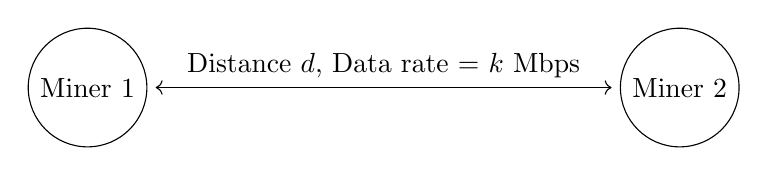
\begin{tikzpicture}
        % Define the nodes
        \node[draw, circle] (node1) {Miner 1};
        \node[draw, circle, right=6cm of node1] (node2) {Miner 2};
        
        % Draw the link
        \draw[<->, shorten >=3pt, shorten <=3pt] (node1) -- node[above] {Distance $d$, Data rate = $k$ Mbps} (node2);
    \end{tikzpicture}   
\end{center}
When miner 1 computes a block and want to transmit to miner 2 the delay is $\frac{d}{c}+\frac{b}{k}$, where b is the length of block size. Miner 2 verifies the block and broadcast it. \\
So the total time taken for end to end propagation of the block in peer to peer network is given below:
$$\sum_{i=1}^{n}\frac{d_i}{c}+\frac{b}{k_i}+p_i$$
where $p_i$ is the time taken for verification of the block, and the links are selected by the spanning tree algorithm for avoiding multiple transfers.
\subsection{How threshold is set}
Thers should be no situation like some miner solves proof of work while other miner broadcasting his bolck, it may lead to forks and double spend. So threshold is choosen such that each block takes 10 minutes to create. \\
The threshold cannot be constant becuase as the users of bitcoin increase the hashing power increases, so satoshi decided to update threshold every 2 weeks based on hashing power. Users use \textbf{A6} hardware for solving proof of work. This 2 weeks is defined in terms of no of blocks, in 2 weeks roughly 2016 blocks were created. \\
So threshold is updated after every 2016 blocks as follows:
$$threshold = threshold * \frac{T}{1209600}$$
T is Time taken for creation of prev 2016 blocks in sec, T can be found using timestamp in block header as follows:
$$T = timestamp(B_{2016n-1}) - timestamp(B_{2016(n-1)})$$
\subsection{Verification}
Ideally miner should follow \textbf{NTP} for the timestamp while solving proof of work.
\subsubsection{Rules for verification}
Miner accepts the recived block if:
$$t_k > median(t_{k-1},t_{k-2},t_{k-3}...... t_{k-11})$$
$$t_k < 2hours + Netwok adjust time$$
Nwtwok adjust time is defined as sum of miner local time according to NTP plus the median of the offsets with local times of his fellow peers.
\subsection{Deal with forks}
Satoshi's first rules were to slect longest chain if forks are present, if multiple longest chains were present should select the one with less timestamp.
\subsubsection{Chain weight}
If some attacker manages to create longest chain privately and broadcast afte he may kill the honest blocks to avoid this chain weight was used. \\
Chain weight uses the sum of expected work done for all the blocks
in the chain, if it is built using fake timestamps he may get caught.
expected work for creating i'th block is calculated as follows:
$$B_i = \lfloor \frac{2^{256}}{Threshold + 1} \rfloor$$
expected work for creating entire chain is calculated as follows:
$$\sum_{i=1}^{n}B_i$$
\section{Confirmation Time}
The confirmation time in blockchain refers to the amount of time it takes for a transaction to be validated and included in a block on the blockchain. The specific confirmation time can vary depending on the blockchain network and its consensus mechanism.\\
\textbf{Zero Confirmation}: A transaction that has been broadcasted but not yet added to a block or confirmed by the network.\\
\textbf{First Confirmation}: The first block in which a transaction is included, indicating its confirmation on the blockchain.\\
\textbf{Second Confirmation}: The second block in which a transaction is included, further validating its confirmation on the blockchain and increasing the level of confidence in its permanence.
\newpage
\begin{figure}
\centering
  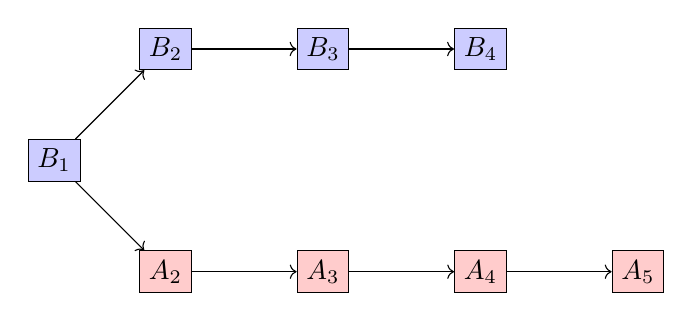
\begin{tikzpicture}[node distance=2cm, auto]
    % Nodes
    \node [draw, rectangle, fill=blue!20] (block1) {$B_1$};
    \node [draw, rectangle, fill=blue!20, above right of=block1] (block2) {$B_2$};
    \node [draw, rectangle, fill=blue!20, right of=block2] (block3) {$B_3$};
    \node [draw, rectangle, fill=blue!20, right of=block3] (block4) {$B_4$};

    \node [draw, rectangle, fill=red!20, below right of=block1] (a2) {$A_2$};
    \node [draw, rectangle, fill=red!20, right of=a2] (a3) {$A_3$};
    \node [draw, rectangle, fill=red!20, right of=a3] (a4) {$A_4$};
    \node [draw, rectangle, fill=red!20, right of=a4] (a5) {$A_5$};

    % Arrows
    \draw [->] (block1) -- (block2);
    \draw [->] (block2) -- (block3);
    \draw [->] (block3) -- (block4);
    \draw [->] (block1) -- (a2);
    \draw [->] (a2) -- (a3);
    \draw [->] (a3) -- (a4);
    \draw [->] (a4) -- (a5);
  \end{tikzpicture}
\end{figure}
\subsection{Double spend attack}
This attack was analysed by Satoshi himself, the above diagram shows the attack after $B_1$, so attacker creates another chain privately after $B_1$ to create double spend and kill the chain created by honest miners. \\
He creates until the other user confirms, i.e if the user waits till 3rd confirmation and attacker broadcast the transaction between $B_1$ and $B_2$, so the user checks if it is in $B_4$ are not, so attacker releases the chain after $A_5$ is created before $b_5$, otherwise he may not.
\begin{center}
\begin{tikzpicture}
    \coordinate (start) at (0,0); % Starting point
    \coordinate (end) at (6,0); % Ending point
    
    % Add height to the first and last coordinate
    \coordinate (p1) at (start |- 0,2);
    \coordinate (p2) at (end |- 0,2);
    
    \draw (p1) -- (start) -- (end) -- (p2); % Draw the line with added height
    
    \pgfmathsetmacro{\n}{5} % Number of divisions
    
    \foreach \i in {2,...,\n}{
        \pgfmathsetmacro{\x}{(\i-1)/\n*6} % Calculate the x-coordinate for each division point
        \coordinate (division\i) at (\x,0); % Store the division point as a coordinate
        \draw (division\i) -- +(0,0.22); % Draw a vertical line indicating the division
        \pgfmathsetmacro{\x}{\i-1}
        \node[below] at (division\i) {$\x*\delta$}; % Label each division point
    }
    
    % Label the first and last coordinates
    \node[above] at (p1) {$B_K$};
    \node[above] at (p2) {$B_{K+1}$};
\end{tikzpicture}
\end{center}
\subsubsection{Inter arrival time of blocks}
We want the distribution of seperation time between each block, let us say that we divided time into intervals of $\delta$ each and $\beta$ is hashing power available. \\
The probabilty that a block is created in the time interval $\delta$ is $\beta\delta$, let us denote the inter arrival time as I so,
$$P[I = n\delta ] = (1 - \beta\delta)^{n-1}\beta\delta$$
$$P[I > n\delta ] = (1 - \beta\delta)^{n}$$
set $n\delta$ as x
$$P[I > x ] = (1 - \frac{\beta*x}{n})^{n}$$
as n goes to $\infty$
$$P[I > x ] = e^{-\beta*x}$$
\subsubsection{Exponential distribution}
The PDF is
$$P[I = x ] = \beta*e^{-\beta*x}$$
The mean or expected value of the distribution is 
$$E[x] = \frac{1}{\beta}$$
This distribution satisfies memoryless property
$$P(X>t+s | X>t)=P(X>s)$$
This property states that the probability of the random variable X exceeding a given threshold t+s, given that it has already exceeded t, is equal to the probability of X exceeding s. \\
From this we can conclude that when the transaction is broadcasted to the miners we should wait for $\frac{1}{\beta}$ which is roughly 10 minutes.
\subsubsection{Poisson arrival process}
The number of blocks created in an interval of T is suprisingly poisson distribution given as 
$$P\left( A_{T} = n \right) = \frac{{e^{ - \beta*t } (\beta *t) ^n }}{{n!}}$$
\subsection{ 51\% Attack}
let p be the fraction of hashing power with honest miners, $q = 1 - p $ be the hashing power with attackers, if $q > 0.5$ then attacker can always kill the chain of honest block.This attack is know as 51\% attack. \\
The naive solution of this attack is to crete checkpoints is that slect a block which is deep enough in the chain must be present in the chain always, checkpoints are updated during a period of time. \\
It is very difficult to acheive more than 50\% of hashing power.
if attacker creates after time y and honest miner after x then probabilty of attacker winning the game is:
\begin{align*}
    P[y < x] &= \int_{0}^{\infty} (1-e^{-\beta*q*x})\beta*p*e^{-\beta*p*x} \, dx\\
      &= \int_{0}^{\infty}\beta*p*e^{-\beta*p*x} \, dx - \int_{0}^{\infty} \beta*p*e^{-\beta*x} \, dx \\
      &= 1 - p \\
      & = q
\end{align*}
\section{Satoshi's analysis}
We want to know the number of confirmations user should wait such that his transaction will be in the blockchain forever. \\
When the transaction is about to enter the block chain attacker may be ahead or behind the honest miners.\\
If attacker is behind the honest miners he should try create more blocks to kill the honest chain, if is ahead he will be wait until the transaction entered the block and releases the chain.\\
\begin{figure}
\centering
  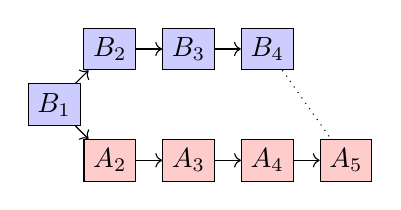
\begin{tikzpicture}[node distance=1cm, auto]
    % Nodes
    \node [draw, rectangle, fill=blue!20] (block1) {$B_1$};
    \node [draw, rectangle, fill=blue!20, above right of=block1] (block2) {$B_2$};
    \node [draw, rectangle, fill=blue!20, right of=block2] (block3) {$B_3$};
    \node [draw, rectangle, fill=blue!20, right of=block3] (block4) {$B_4$};

    \node [draw, rectangle, fill=red!20, below right  of=block1] (a2) {$A_2$};
    \node [draw, rectangle, fill=red!20, right of=a2] (a3) {$A_3$};
    \node [draw, rectangle, fill=red!20, right of=a3] (a4) {$A_4$};
    \node [draw, rectangle, fill=red!20, right of=a4] (a5) {$A_5$};
    % Arrows
    \draw [->] (block1) -- (block2);
    \draw [->] (block2) -- (block3);
    \draw [->] (block3) -- (block4);
    \draw [->] (block1) -- (a2);
    \draw [->] (a2) -- (a3);
    \draw [->] (a3) -- (a4);
    \draw [->] (a4) -- (a5);
    \draw [dotted] (block4) -- (a5);
  \end{tikzpicture}
  \caption{attacker is ahead of honest miners}
\end{figure}
\begin{figure}
\centering
  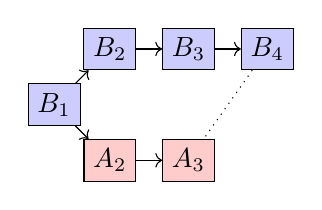
\begin{tikzpicture}[node distance=1cm, auto]
    % Nodes
    \node [draw, rectangle, fill=blue!20] (block1) {$B_1$};
    \node [draw, rectangle, fill=blue!20, above right of=block1] (block2) {$B_2$};
    \node [draw, rectangle, fill=blue!20, right of=block2] (block3) {$B_3$};
    \node [draw, rectangle, fill=blue!20, right of=block3] (block4) {$B_4$};

    \node [draw, rectangle, fill=red!20, below right of=block1] (a2) {$A_2$};
    \node [draw, rectangle, fill=red!20, right of=a2] (a3) {$A_3$};
    % Arrows
    \draw [->] (block1) -- (block2);
    \draw [->] (block2) -- (block3);
    \draw [->] (block3) -- (block4);
    \draw [->] (block1) -- (a2);mining on his block
    \draw [->] (a2) -- (a3);
    \draw [dotted] (block4) -- (a3);
  \end{tikzpicture}
  \caption{attacker is behind the honest miners}
\end{figure}
Satoshi assumed that network delay is zero and observed the attacker's lead with time.
\begin{center}
\begin{tikzpicture}
  % Draw x-axis
  \draw[->] (0,0) -- (11,0) node[right] {time};
  
  % Draw y-axis with label
  \draw[->] (0,0) -- (0,6) node[above] {Attackers lead};
  
  % Draw your points and join them with straight lines
  \draw plot[const plot, mark=*, mark size=2pt] coordinates{(0,1) (1,2) (2,1) (3,3) (4,2)(5,6)(6,5)(7,4)(8,3)(9,2)(10,0)};
  \node[above right] at (5,6) {$Z$};
  \node[above right] at (5,0) {$S$};
  \node[above right] at (10,0) {$A$};
  % Draw the dotted line
  \draw[dotted] (5,0) -- (5,5);
\end{tikzpicture}
\end{center}
From the above picture Z can be in the range $(-\infty, S)$, where S is indicating S'th confirmation, we also have to see after S if he can win at some point like A in above in future. S, A location is variable it can happen anywhere and it affects the value of Z.
\subsection{Meni Rosenfeld discrete analysis}
We will be marking points at which blocks were created and observe it when S number of blocks are created by honest miners.
\begin{center}
    \begin{tikzpicture}
  % Draw x-axis
  \draw[-latex] (0,0) -- (7,0) node[right] {$Time$};

% Add text above x-axis
  \node[above] at (0,2) {Honest};
  
  % Add text below x-axis
  \node[below] at (0,-2) {Attacker};
  
  % Draw lines in positive y-direction
  \draw (1,0) -- (1,2);
  \draw (2,0) -- (2,2);
  \draw (4,0) -- (4,2);
  
  % Draw lines in negative y-direction
  \draw (3,0) -- (3,-2);
  \draw (5,0) -- (5,-2);
  \draw (6,0) -- (6,2);
  
  % Add label "S" for the last line in positive y-direction
  \draw (6,0) -- (6,2) node[midway, right] {S};
  \draw (5,0) -- (5,-2) node[midway, right] {X};
\end{tikzpicture}
\end{center}
If the honest miners are ahead of Z blocks at the S'th confirmation,
$$X = S - Z$$
we have to calculate the probabilty that honest miners have lead Z  at S'th confirmation, 
$$P_{Z,S} = Prob((S -X = Z) | (Honest = S) )$$
Also the attacker catching up the lead Z as $Q_{Z}$. \\
Probability that attacker catches up after S honest blocks,
$$R_{S} = \sum_{-\infty}^{S}P_{Z,S}*Q_{Z}$$
$$P_{Z,S} = \binom{2*S - Z - 1}{S - 1}*P^{S}*Q^{S-Z}$$
For finding $Q_Z$ we should perform random walk as there are many possibilities to catch up the lead, this can analysed by an simple automeata as below, 
\begin{center}
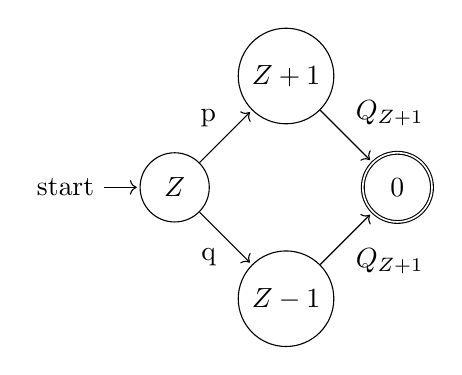
\begin{tikzpicture}[shorten >=1pt,node distance=2cm,on grid,auto] 
   \node[state,initial] (q_0)   {$Z$}; 
   \node[state] (q_1) [above right=of q_0] {$Z+1$}; 
   \node[state] (q_2) [below right=of q_0] {$Z-1$}; 
   \node[state,accepting](q_3) [below right=of q_1] {$0$};
    \path[->] 
    (q_0) edge  node {p} (q_1)
          edge  node [swap] {q} (q_2)
    (q_1) edge  node  {$Q_{Z+1}$} (q_3)
    (q_2) edge  node [swap] {$Q_{Z+1}$} (q_3) ;
\end{tikzpicture}    
\end{center}
So for $Z > 0$,
$$Q_Z = P*Q_{Z+1} + q*Q_{Z-1}$$
on solving, 
\[
Q_{Z} =
\begin{cases}
(\frac{q}{p})^{Z} & \text{if } Z \geq 0 \\
1 & \text{if } Z < 0 \\
\end{cases}
\]
The above $Q_{Z}$ is only true if $ q < p $, else $Q_{Z}$ is always 1 which leads to 51\% attack.
\section{Selfish mining}
Selfish mining is a strategy where a miner intentionally withholds mined blocks to gain a competitive advantage and disrupt the fairness of the blockchain network. To perform selfish mining we should have an reasonable amount of hashing power.
\subsection{Majority is not enough}
This attack was analysed by Eyal and Siral around 2015. \\
If the block is created by honest miner before attacker creates a block, all the miners including attackers starts mining on this block as shown in figure 3.\\
\begin{figure}
\centering
  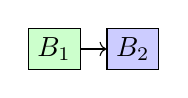
\begin{tikzpicture}[node distance=1cm, auto]
    % Nodes
    \node [draw, rectangle, fill=green!20] (block1) {$B_1$};
    \node [draw, rectangle, fill=blue!20, right of=block1] (block2) {$B_2$};
    % Arrows
    \draw [->] (block1) -- (block2);
  \end{tikzpicture}
  \caption{honest miners creates first}
\end{figure}
If the attacker creates he waits and if the honest miner also creates some time after, if attacker has no lead he releases the block which leads all the attackers and some fraction of honest miners mining on his block, remaining fraction on honest block, as shown in figure 4.
If $B_3$ is created first attacker chain is killed, similarly if $b_3$ or $A_3$ is created the honest miners chain is killed.\\ 
\begin{figure}
\centering
  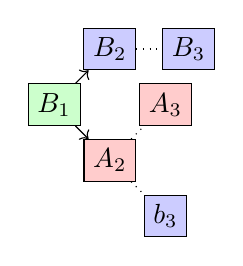
\begin{tikzpicture}[node distance=1cm, auto]
    % Nodes
    \node [draw, rectangle, fill=green!20] (block1) {$B_1$};
    \node [draw, rectangle, fill=blue!20, above right of=block1] (block2) {$B_2$};
    \node [draw, rectangle, fill=blue!20, right of=block2] (block3) {$B_3$};
    \node [draw, rectangle, fill=red!20, below right of=block1] (a2) {$A_2$};
    \node [draw, rectangle, fill=red!20, above right of=a2] (a3) {$A_3$};
    \node [draw, rectangle, fill=blue!20, below right of=a2] (b3) {$b_3$};
    \draw [->] (block1) -- (block2);
    \draw [dotted] (block2) -- (block3);
    \draw [->] (block1) -- (a2);
    \draw [dotted] (a2) -- (b3);
    \draw [dotted] (a2) -- (a3);
  \end{tikzpicture}
  \caption{attacker and honest miners release simultaneously}
\end{figure}
So if attacker had a lead 2 or more he waits until lead becomes 1 and releases the chain and kill the honest chain, each attacker block gets lead but not the honest blocks in this case attacker releases the chain as $B_4a$ was created before $A_6$ as shown in figure 5.
\begin{figure}
\centering
  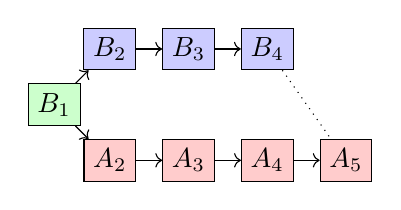
\begin{tikzpicture}[node distance=1cm, auto]
    % Nodes
    \node [draw, rectangle, fill=green!20] (block1) {$B_1$};
    \node [draw, rectangle, fill=blue!20, above right of=block1] (block2) {$B_2$};
    \node [draw, rectangle, fill=blue!20, right of=block2] (block3) {$B_3$};
    \node [draw, rectangle, fill=blue!20, right of=block3] (block4) {$B_4$};

    \node [draw, rectangle, fill=red!20, below right of=block1] (a2) {$A_2$};
    \node [draw, rectangle, fill=red!20, right of=a2] (a3) {$A_3$};
    \node [draw, rectangle, fill=red!20, right of=a3] (a4) {$A_4$};
    \node [draw, rectangle, fill=red!20, right of=a4] (a5) {$A_5$};
    % Arrows
    \draw [->] (block1) -- (block2);
    \draw [->] (block2) -- (block3);
    \draw [->] (block3) -- (block4);
    \draw [->] (block1) -- (a2);
    \draw [->] (a2) -- (a3);
    \draw [->] (a3) -- (a4);
    \draw [->] (a4) -- (a5);
    \draw [dotted] (block4) -- (a5);
  \end{tikzpicture}
  \caption{all the attacker blocks get into the chain}
\end{figure}
\newpage
\subsection{Markov chain}
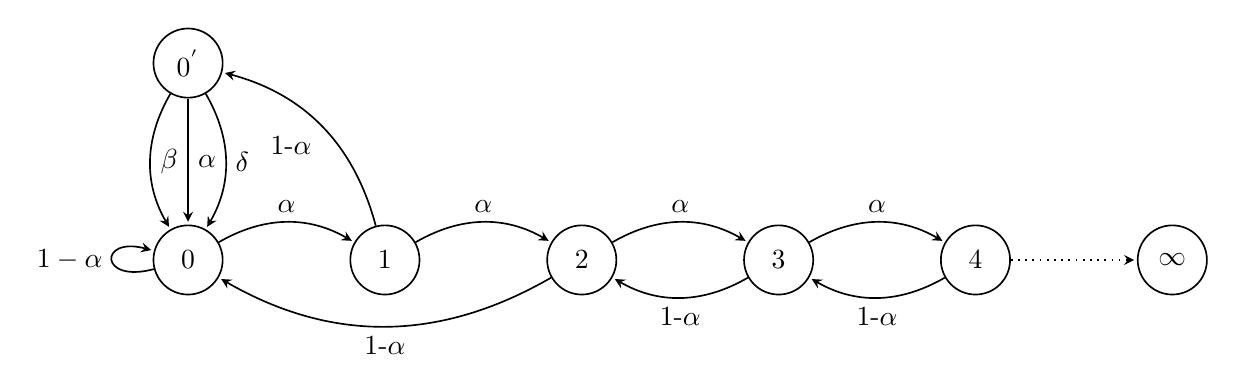
\begin{tikzpicture}[->,>=stealth,shorten >=1pt,auto,node distance=2.5cm,semithick]
    \node[state,circle] (0) {$0$};
    \node[state,circle] (0*) [above of=0]{$0^{'}$};
    \node[state,circle] (1)[right of=0] {$1$};
  \node[state,circle] (2) [right of=1]{$2$};
  \node[state,circle] (3) [right of=2] {$3$};
  \node[state,circle] (4) [right of=3] {$4$};
  \node[state,circle] (5) [right of=4] {$\infty$};
  \path (2) edge [bend left] node {$\alpha$} (3)
        (0) edge [loop left] node {$1-\alpha$} (0)
        (0) edge [bend left] node {$\alpha$} (1)
        (1) edge [bend left] node {$\alpha$} (2)
        (0*) edge [bend left] node {$\delta$} (0)
        (0*) edge [bend right] node {$\beta$} (0)
        (0*) edge  node {$\alpha$} (0)
        (1) edge [bend right] node {1-$\alpha$} (0*)
        (3) edge [bend left] node {1-$\alpha$} (2)
        (2) edge [bend left] node {1-$\alpha$} (0)
        (3) edge [bend left] node {$\alpha$} (4)
        (4) edge [bend left] node {1-$\alpha$} (3)
        (4) edge [dotted] (5);
\end{tikzpicture}
$$\beta = (1-\alpha)(1-\gamma)$$
$$\delta = (1-\alpha)\gamma$$
According to the paper attacker gets one block in each $(i,i+1)$, 2 blocks in (2,0) state change, honest miner may get 1,2 or 0 blocks in $(0^{'},0)$ state change depending on who creates the block.
\subsection{Discrete time markove chain analysis}
\begin{center}
 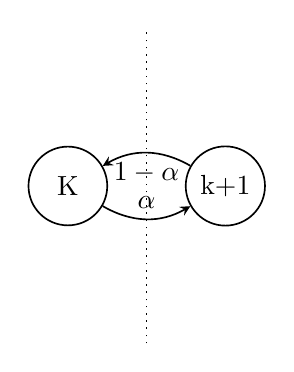
\begin{tikzpicture}[>=stealth, auto, node distance=2cm, on grid, semithick, every state/.style={minimum size=1cm}]
  \node[state] (A) {K};
  \node[state] (B) [right=of A] {k+1};
  
  \path[->] (A) edge[bend right] node {$\alpha$} (B);
  \path[->] (B) edge[bend right] node {$1-\alpha$} (A);

  \draw[dotted] (1,-2) -- (1,2); % Vertical dotted line
\end{tikzpicture} 
\end{center}
From the above figure if we make an vertical cut the flow should be equal from both sides in steady state so for $k \geq 2$,
$$P_{k}*\alpha = P_{k+1}*(1-\alpha)$$
make cut between 1 and $0^{'}$, 0 and 1,
$$P_{0^{'}} = P_{1}*(1-\alpha)$$
$$P_{0} = (P_{1}+ P_{2})*(1-\alpha)$$
on solving,
$$P_{0} = \frac{\alpha - 2*\alpha^{2}}{\alpha*(2*\alpha^{3} - 4*\alpha^{2} + 1)}$$
$$P_{0^{'}} = \frac{(1-\alpha)*(\alpha - 2*\alpha^{2})}{2*\alpha^{3} - 4*\alpha^{2} + 1}$$
$$P_{1} = \frac{\alpha - 2*\alpha^{2}}{2*\alpha^{3} - 4*\alpha^{2} + 1}$$
for all $k \geq 2$,
$$P_{k} = (\frac{\alpha}{1-\alpha})^{k-1}*(\frac{\alpha - 2*\alpha^{2}}{2*\alpha^{3} - 4*\alpha^{2} + 1})$$
\subsection{Rewards}
$r_{pool}$ is defined as ratio of number of attacker blocks entered(A) int to final chain to the sum of all blocks generated by attacker($A_0$) and honest miners($H_0$). \\
$$r_{pool} = \frac{A}{A_0 + H_0}$$
$$r_{others} = \frac{H}{A_0 + H_0}$$
$$\frac{r_{pool}}{r_{pool}+r_{others}} = \frac{A}{A + H}$$
$$r_{others} = P_{0^{'}}*(1-\alpha)*\gamma + P_{0^{'}}*(1-\alpha)*(1-\gamma)*2 + P_{0}*(1-\alpha)$$
$$r_{pool} = P_{0^{'}}*(1-\alpha)*\gamma + P_{0^{'}}*2*\gamma + P_{2}*(1-\alpha)*2 + \sum_{2}^{\infty}P_{i}*\alpha$$
$$R_{pool} = \frac{A}{A + H}$$
$$R_{pool} = \frac{\alpha*(1-\alpha)^{2}*(4*\alpha + \gamma(1-2*\alpha))-\alpha^{3}}{1-\alpha*(1+(2-\alpha))*\alpha}$$
Where $\alpha$ is hashing power of attackers pool and $\gamma$ is the fraction of honest miners who follow attackers after releasing attackers chain. \\
In the context of Bitcoin, a mining pool is a group of miners who come together to combine their computing power and resources in order to increase their chances of successfully mining new blocks and earning Bitcoin rewards. Here's how a mining pool typically operates:
\begin{enumerate}
\item Miners join the pool: Individual miners join a mining pool by connecting their mining hardware (such as specialized computers called ASICs) to the pool's mining server.

\item Solving hash puzzles: The mining pool's server assigns computational tasks to the connected miners, typically in the form of hash puzzles.

\item Work distribution: The pool's server distributes different variations of the hash puzzle to the connected miners.

\item Finding a block: Once a miner in the pool successfully solves a hash puzzle, they broadcast the solution to the pool's server.

\item Distribution of rewards: Rewards are distributed among pool participants based on the proportion of hashing power they contributed.

\item Continuous mining: Miners in the pool continue to receive new hash puzzles and work on solving them to find more blocks and earn rewards.
\end{enumerate}
\section{Proof Of Stake}
\subsection{Sybil attack}
In a blockchain, a Sybil attack involves an attacker claims to have more hashing power than what he actually have. \\
In proof of work Sybil attack cannot be performed because someone cannot fake real time work done by them, but the problem with proof of work is it consumes more energy.\\
Proof of stake(PoS) is a consensus protocol unlike Proof of Work (PoW), which relies on miners solving complex mathematical puzzles, PoS selects validators to create and validate new blocks based on the amount of cryptocurrency they hold and "stake" as collateral.\\ 
Proof of work uses hash of previous block, nonce(IV), timestamp(T), merkle root of the transactions(MR) to solve the puzzle as follows,
\begin{equation*}
    Hash(Hash(B_{k}),IV,T,MR, ....) < Threshold
\end{equation*}
Proof of stake uses the hash of previous block, public key(a), balance with a, timestamp and merkle root is not included, but the threshold is varied for miners because people with more stake should have more chance, also timestamp should be near to local time. \\
\begin{equation*}
    Hash(Hash(B_{k}),a,T, ....) < Threshold*balance(a)
\end{equation*}
\subsection{Nothing at stake}
The "nothing at stake" problem is a concern in Proof of Stake (PoS) blockchains where validators have no financial disincentive to support multiple conflicting forks. Since PoS validators are not required to spend computational resources to mine blocks, they can potentially support all competing chains simultaneously. This lack of economic cost removes the incentive to converge on a single valid chain, leading to a lack of consensus. To mitigate this problem, PoS protocols implement penalties or slashing conditions to discourage validators from supporting multiple forks, ensuring network stability and security.
\begin{figure}
\centering
  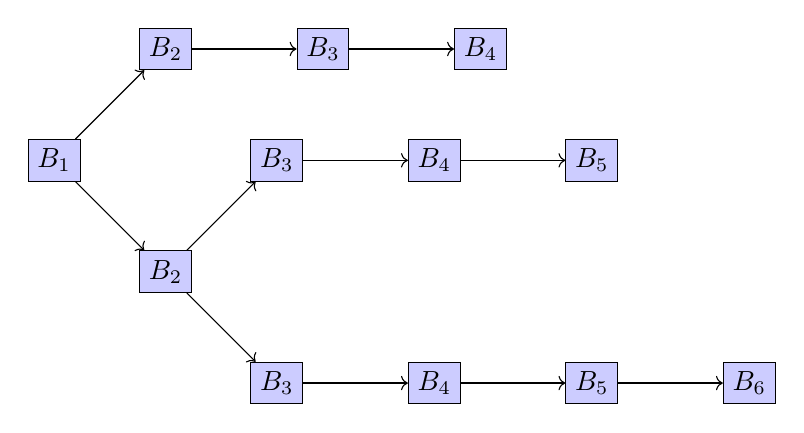
\begin{tikzpicture}[node distance=2cm, auto]
    % Nodes
    \node [draw, rectangle, fill=blue!20] (block1) {$B_1$};
    \node [draw, rectangle, fill=blue!20, above right of=block1] (block2) {$B_2$};
    \node [draw, rectangle, fill=blue!20, right of=block2] (block3) {$B_3$};
    \node [draw, rectangle, fill=blue!20, right of=block3] (block4) {$B_4$};

    \node [draw, rectangle, fill=blue!20, below right of=block1] (a2) {$B_2$};
    \node [draw, rectangle, fill=blue!20, above right of=a2] (a3) {$B_3$};
    \node [draw, rectangle, fill=blue!20, right of=a3] (a4) {$B_4$};
    \node [draw, rectangle, fill=blue!20, right of=a4] (a5) {$B_5$};
    \node [draw, rectangle, fill=blue!20, below right of=a2] (b2) {$B_3$};
    \node [draw, rectangle, fill=blue!20, right of=b2] (b3) {$B_4$};
    \node [draw, rectangle, fill=blue!20, right of=b3] (b4) {$B_5$};
    \node [draw, rectangle, fill=blue!20, right of=b4] (b5) {$B_6$};
    % Arrows
    \draw [->] (block1) -- (block2);
    \draw [->] (block2) -- (block3);
    \draw [->] (block3) -- (block4);
    \draw [->] (block1) -- (a2);
    \draw [->] (a2) -- (a3);
    \draw [->] (a3) -- (a4);
    \draw [->] (a4) -- (a5);
    \draw [->] (a2) -- (b2);
    \draw [->] (b2) -- (b3);
    \draw [->] (b3) -- (b4);
    \draw [->] (b4) -- (b5);
  \end{tikzpicture}
  \caption{Nothing at stake attack}
\end{figure}
\subsection{Long range attack}
A long-range attack is a security concern in blockchain systems, where an attacker attempts to rewrite the entire blockchain's history. By possessing a significant amount of stake or historical data, the attacker creates an alternative chain from an earlier point in time to surpass the current valid chain. This can invalidate previous transactions and compromise the integrity of the network as shown in figure 7.
\begin{figure}
\centering
  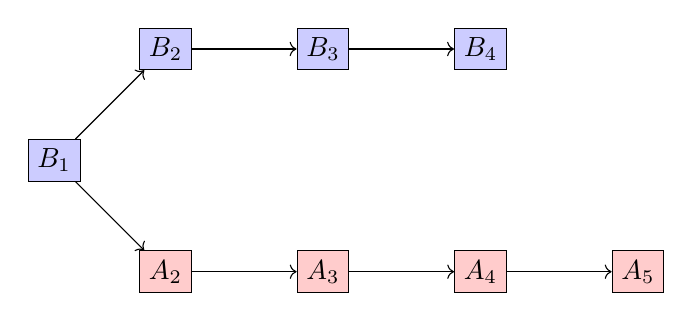
\begin{tikzpicture}[node distance=2cm, auto]
    % Nodes
    \node [draw, rectangle, fill=blue!20] (block1) {$B_1$};
    \node [draw, rectangle, fill=blue!20, above right of=block1] (block2) {$B_2$};
    \node [draw, rectangle, fill=blue!20, right of=block2] (block3) {$B_3$};
    \node [draw, rectangle, fill=blue!20, right of=block3] (block4) {$B_4$};

    \node [draw, rectangle, fill=red!20, below right of=block1] (a2) {$A_2$};
    \node [draw, rectangle, fill=red!20, right of=a2] (a3) {$A_3$};
    \node [draw, rectangle, fill=red!20, right of=a3] (a4) {$A_4$};
    \node [draw, rectangle, fill=red!20, right of=a4] (a5) {$A_5$};

    % Arrows
    \draw [->] (block1) -- (block2);
    \draw [->] (block2) -- (block3);
    \draw [->] (block3) -- (block4);
    \draw [->] (block1) -- (a2);
    \draw [->] (a2) -- (a3);
    \draw [->] (a3) -- (a4);
    \draw [->] (a4) -- (a5);
  \end{tikzpicture}
  \caption{Long range attack killing blue chain after $B_1$}
\end{figure}
HAs stake goes up so attacker might approach real time in creating blocks i.e creating bloks at every 10 minutes and he can easily kill the entire chain easily.
\subsection{Initial distribution problem}
The initial distribution problem in Proof of Stake (PoS) refers to the challenge of fairly allocating cryptocurrency among participants at the launch of a PoS blockchain. Concentration of stake by early adopters can lead to centralization and disproportionate control. Strategies like fair token distribution and airdrops are used to promote decentralization and prevent dominance by a few stakeholders.
\subsection{Bribe attack}
A bribe attack is a type of attack where an adversary attempts to manipulate the behavior of participants in a blockchain network by offering them incentives or bribes. The attacker aims to persuade participants to act in a way that benefits the attacker's interests. This attack can undermine the integrity and security of the blockchain consensus. Countermeasures include promoting transparency, strong governance mechanisms, and encouraging participants to act in the best interest of the network rather than personal gain.
\subsection{Pre computing attack}
A pre-computing attack in Proof of Stake (PoS) refers to a potential attack where an adversary tries to gain an unfair advantage by pre-computing a large number of block proposals or validations before they are actually required. By pre-computing blocks as he can change the transaction anytime in previous block, the attacker can quickly gain control over the blockchain and influence the consensus process.
\section{Hybrid PoW and PoS consensus}
Use proof of work but not too much of energy i.e don't use proof of work in every block, also use proof of stake for consensus protocol.
The proposed hybris solution is use PoW after every N blocks in between use Pos as shown in figure 8. \\
By using this the PoW energy per unit time is changed to $\frac{M}{NT}$ from $\frac{M}{T}$ where M is mining fee per block and T ia average time per creating a block.
\begin{figure}
\centering
  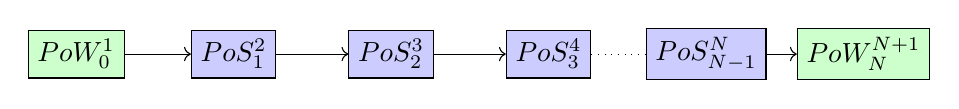
\begin{tikzpicture}[node distance=2cm, auto]
    % Nodes
    \node [draw, rectangle, fill=green!20] (block1) {$PoW_{0}^1$};
    \node [draw, rectangle, fill=blue!20, right of=block1] (block2) {$PoS_{1}^2$};
    \node [draw, rectangle, fill=blue!20, right of=block2] (block3) {$PoS_{2}^3$};
    \node [draw, rectangle, fill=blue!20, right of=block3] (block4) {$PoS_{3}^4$};
    \node [draw, rectangle, fill=blue!20, right of=block4] (block5) {$PoS_{N-1}^N$};
    \node [draw, rectangle, fill=green!20, right of=block5] (block6) {$PoW_{N}^{N+1}$};

    % Arrows
    \draw [->] (block1) -- (block2);
    \draw [->] (block2) -- (block3);
    \draw [->] (block3) -- (block4);
    \draw [dotted] (block4) -- (block5);
    \draw [->] (block5) -- (block6);
  \end{tikzpicture}
  \caption{Hybrid solution}
\end{figure}
\section{SLASHER}
The concept of "slasher" was proposed by Vitalik Buterin, the co-founder of Ethereum. Slasher is a type of consensus mechanism that was introduced as an alternative to the traditional Proof-of-Work (PoW) algorithm used by Bitcoin. Slasher focuses on penalizing validators who act dishonestly or attempt to manipulate the blockchain.\\
Reducing mining reward which could potentially reduce the overall computational power and energy consumption required for mining operations. \\
In slasher each valid block is signed by some group of people selected by proof osf stake beforehand and created by proof of work, so double spend attack is non trivial as attacker should create blocks with PoW and should have signatures. \\
As shown in figure 9 the blocks are signed by designated signers after the creation of the block, if any person signs multiple blocks at the same level of the fork he will be penalized. \\
All the signers selected by PoS has to deposit stake for some duration. The stake is frozen during the time i.e from $B_k$ to $B_{k+n}$ block. If anyone cheats during the time the stake is confiscated by creating a punishment transaction which involves some part to the user who created the transaction, miner who includes the transaction as shown in figure 10.
$\alpha, \beta$ are in range $(0,1)$ so the part of money paid to shared key 0 is burnt.
\begin{figure}
\centering
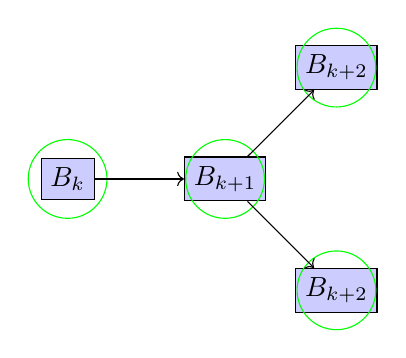
\begin{tikzpicture}[node distance=2cm, auto]
  % Nodes
  \node [draw, rectangle, fill=blue!20] (block1) {$B_{k}$};
  \node [draw, rectangle, fill=blue!20, right of=block1] (block2) {$B_{k+1}$};
  \node [draw, rectangle, fill=blue!20, above right of=block2] (block3) {$B_{k+2}$};
  \node [draw, rectangle, fill=blue!20, below right of=block2] (block4) {$B_{k+2}$};

  % Circles
  \foreach \node in {block1, block2, block3, block4}
    \draw [green] (\node) circle (0.5cm);

  % Arrows
  \draw [->] (block1) -- (block2);
  \draw [->] (block2) -- (block3);
  \draw [->] (block2) -- (block4);
\end{tikzpicture}
\caption{Signing the blocks}
\end{figure}
\begin{figure}
    \centering
\begin{center}
\begin{tikzpicture}[>={Latex[scale=1]}]
  %% Encoder
  \node (naveq) [naveqs] {Transaction};
  %% Inputs
  \draw[<-] ($(naveq.south west)!0.5!(naveq.north west)$) -- +(-\edgedist,0) node [left] {$PK^{i}_0$}
  node[midway,above] {$X$};;
  %% Outputs
  \draw[->] ($(naveq.south east)!0.6!(naveq.north east)$) -- +(\edgedist,0) node [right] {$PK^{o}_0$} node[midway,above] {$\alpha*X$};
  \draw[->] ($(naveq.south east)!0.3!(naveq.north east)$) -- +(\edgedist,0) node [right] {$0$} node[midway,below] {$(1-\beta)*\alpha*X$};
\end{tikzpicture}
\end{center}
    \caption{punishment transaction}
\end{figure}
\begin{figure}
\centering
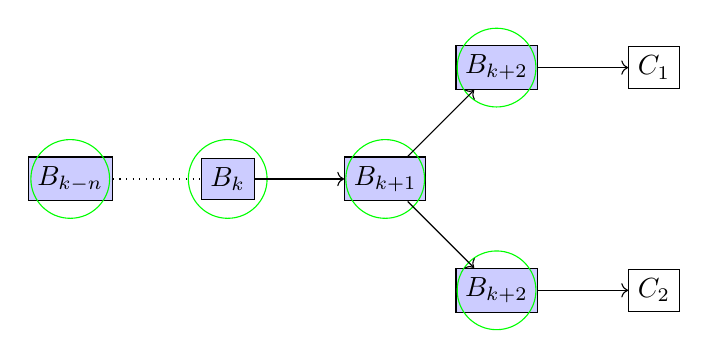
\begin{tikzpicture}[node distance=2cm, auto]
  % Nodes
  \node [draw, rectangle, fill=blue!20] (block0) {$B_{k-n}$};
  \node [draw, rectangle, fill=blue!20, right of =block0] (block1) {$B_{k}$};
  \node [draw, rectangle, fill=blue!20, right of=block1] (block2) {$B_{k+1}$};
  \node [draw, rectangle, fill=blue!20, above right of=block2] (block3) {$B_{k+2}$};
  \node [draw, rectangle, fill=blue!20, below right of=block2] (block4) {$B_{k+2}$};
  \node [draw, rectangle,  right of=block3] (block5) {$C_{1}$};
  \node [draw, rectangle,  right of=block4] (block6) {$C_2$};

  % Circles
  \foreach \node in {block0, block1, block2, block3, block4}
    \draw [green] (\node) circle (0.5cm);

  % Arrows
  \draw[dotted](block0) -- (block1);
  \draw [->] (block1) -- (block2);
  \draw [->] (block2) -- (block3);
  \draw [->] (block2) -- (block4);
  \draw [->] (block3) -- (block5);
  \draw [->] (block4) -- (block6);
\end{tikzpicture}
\caption{selecting multiple committee at forks}
\end{figure}
\subsection{Rules for signing}
A group signers are selected for signing $B_{K+M}$ at $B_{K}$ using proof of stake, assuming that a large number of these signers are honest, a block is valid if and only if it has at least $\frac{2}{3}$ group signatures, the group is called as committee to sign.
\subsection{Choosing the committee}
If the committee for $B_{k}$ is selected as $B_{k-1}$ there is a chance of selecting two committee if a fork is present as shown in figure 11, so we go deep into the block chain and select the committee as there is a less chance that there is a long fork from the deep enough block.
\subsection{Slasher rules}
\begin{itemize}
    \item Blocks are mined using PoW, mining reward decreases by a factor of 50 every year.
    \item Every block has set of designated signers choosed beforehand.
    \item A block is valid if it has more than $\frac{2}{3}$ of signatures from the designated signers.
\end{itemize}
\subsection{Potential signers}
When $B_k$ is produced the potential signers of block $B_{k+3000}$ are those with address a,
$$Hash(a, Hash(B_k)) < bal(a)*Target$$
we need about 15 potential signers to volunteer to become designated signers, so Target is adjusted such that abou 15 people volunteer every time.
\begin{figure}
\centering
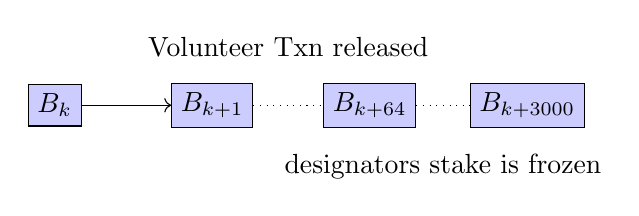
\begin{tikzpicture}[node distance=2cm, auto]
  % Nodes
  \node [draw, rectangle, fill=blue!20] (block0) {$B_{k}$};
  \node [draw, rectangle, fill=blue!20, right of =block0] (block1) {$B_{k+1}$};
  \node [draw, rectangle, fill=blue!20, right of=block1] (block2) {$B_{k+64}$};
  \node [draw, rectangle, fill=blue!20, right of=block2] (block3) {$B_{k+3000}$};
  % Arrows
  \draw[->](block0) -- (block1);
  \draw [dotted] (block1) -- node[above=0.5cm] {Volunteer Txn released} (block2);
  \draw [dotted] (block2) -- node[below=0.5cm] {designators stake is frozen} (block3);
\end{tikzpicture}
\caption{designated signers selection}
\end{figure}
\section{Designated signers}
Any potential signer of $B_{k+3000}$ can be a designated signer by sending a volunteer transaction between $B_{k+1}$ and $B_{k+64}$, the deposits are frozen from $B_{k+64}$ to $B_{k+6000}$ of the designated signers, there will be no signers fro first 300 blocks.
what if none of the block has $\frac{2}{3}$ signatures or every block has more than $\frac{2}{3}$ signatures then miners should start mining on the parent block by skipping the blocks at the same level. \\
If they skip n blocks then the new threshold will be 
$$Target = Target * 8 * 2^{n-1}$$
\section{Anonimity}
Blockchain provides pseudonymity, where users are identified by cryptographic addresses instead of personal information, but it is not inherently anonymous as transactions can be traced through blockchain analysis techniques.
\subsection{Properties of unlinkability}
\begin{itemize}
    \item Hard to link different addresses of the same user.
    \item Hard to link different transactions of the same user.
    \item Hard to link sender and recipient of the same transaction.
\end{itemize}
\subsection{De-anonymization}
If recipient address is well known then it is easy to track his all transaction as they are part of directed graph. To avoid this users always change their address at each transaction.
\tikzstyle{sensor}=[draw, fill=blue!20, text width=5em, 
text centered, minimum height=2.5em]
\tikzstyle{ann} = [above, text width=6em]
\tikzstyle{naveqs} = [sensor, text width=6em, fill=red!20, 
minimum height=6em, rounded corners]
\def\blockdist{2.3}
\def\edgedist{1}
\begin{center}
\begin{tikzpicture}[>={Latex[scale=0.5]}]
    %% Encoder (First Block)
    \node (naveq) [naveqs] {Transaction 1};
    %% Inputs
    \draw[<-] ($(naveq.south west)!0.75!(naveq.north west)$) -- +(-\edgedist,0) node [left] {$P_{A}$} node [midway,above] {3};
    \draw[<-] ($(naveq.south west)!0.25!(naveq.north west)$) -- +(-\edgedist,0) node [left] {$P_{C}$} node [midway,above] {5};

    %% Decoder (Second Block)
    \node (decoder) [naveqs, right=2cm of naveq] {Transaction 2};
    \draw[->] ($(decoder.south east)!0.75!(decoder.north east)$) -- node[below] {$P_{D}$} node [midway,above] {6} ($(decoder.south east)!0.75!(decoder.north east) + (1.5cm,0)$);
    \draw[->] ($(decoder.south east)!0.25!(decoder.north east)$) -- node[below] {$P_{B_{3}}$} node [midway,above] {2}($(decoder.south east)!0.25!(decoder.north east) + (1.5cm,0)$);

    %% Connection between blocks
    \draw[->] ($(naveq.south east)!0.75!(naveq.north east) + (-0.0625cm,0)$) -- node[above] {$P_{B_{1}}$}node [below] {3}($(decoder.south west)!0.75!(decoder.north west)$);
    \draw[->] ($(naveq.south east)!0.25!(naveq.north east) + (-0.0625cm,0)$) -- node[above] {$P_{B_{2}}$}node [below] {5}($(decoder.south west)!0.25!(decoder.north west)$);
\end{tikzpicture}
\end{center}
In the above transaction show we can easily know the $P_{B_{1}}$, $P_{B_{2}}$ belong to the same user as he is combining them to pay, some wallets by default generates a new change address and keeps it randomly among the outputs to fix this issue, but if there is only one new address among the output then one can de-anonymize them easily. \\
\subsubsection{network de-anonymization}
Network deanonymization in a P2P network means figuring out who is behind the network activities. It can be done through analyzing traffic patterns, creating fake identities, or tracking IP addresses.\\
The Tor network and onion routing are used to enhance privacy by obscuring the origin and destination of network traffic, making it difficult to link Bitcoin transactions to specific individuals.
\subsection{Tor network \& Onion routing}
The Tor network is a decentralized network of volunteer-operated servers that routes internet traffic through multiple layers of encryption and relays to protect user privacy and anonymity.\\
Onion routing is a technique employed by the Tor network where data is encrypted in multiple layers (like the layers of an onion) and routed through a series of relays, with each relay peeling off a layer of encryption, making it challenging to trace the source or destination of the traffic. This helps in preventing network deanonymization in Bitcoin by obscuring the true origin and destination of transactions.
\section{Mixing}
Mixing is done in blockchains to enhance privacy and anonymity. By mixing or combining transactions from different participants, we don't want a mapping between users and their addresses. \\
\tikzstyle{sensor}=[draw, fill=blue!20, text width=5em, 
text centered, minimum height=2.5em]
\tikzstyle{ann} = [above, text width=6em]
\tikzstyle{naveqs} = [sensor, text width=6em, fill=red!20, 
minimum height=6em, rounded corners]
\tikzstyle{naveqs1} = [sensor, text width=6em, fill=blue!20, 
minimum height=10em, rounded corners]
\def\blockdist{2.3}
\def\edgedist{1}
\begin{center}
\begin{tikzpicture}[>={Latex[scale=0.5]}]
    %% Encoder (First Block)
    \node (naveq) [naveqs] {Transaction};
    %% Inputs
    \draw[<-] ($(naveq.south west)!0.5!(naveq.north west)$) -- +(-\edgedist,0) node [left] {$P_{Z}$} node [midway,above] {z};

    %% Decoder (Second Block)
    \node (decoder) [naveqs1, right=2cm of naveq] {Mixer};
    \draw[->] ($(decoder.south east)!0.9!(decoder.north east)$) -- node[below] {$P_{A_{1}}$} node [midway,above] {$a_1$} ($(decoder.south east)!0.9!(decoder.north east) + (1.5cm,0)$);
    \draw[->] ($(decoder.south east)!0.6!(decoder.north east)$) -- node[below] {$P_{A_{2}}$} node [midway,above] {$a_2$}($(decoder.south east)!0.6!(decoder.north east) + (1.5cm,0)$);
    \draw[->] ($(decoder.south east)!0.3!(decoder.north east)$) -- node[below] {$P_{A_{3}}$} node [midway,above] {$a_3$}($(decoder.south east)!0.3!(decoder.north east) + (1.5cm,0)$);

    %% Connection between blocks
    \draw[->] ($(naveq.south east)!0.5!(naveq.north east) + (-0.0625cm,0)$) -- node[above] {$P_{A}$}node [below] {a}($(decoder.south west)!0.5!(decoder.north west)$);
\end{tikzpicture}
\end{center}
In the above picture $P_A$ recieves some money a from $P_Z$, $P_A$ approaches the mixer to split it's money among the public keys provided by himself, mixer take cares that any person other than A know that theys addresses belong to A. We assume that mixers are honest and pay back the money.\\
All the money from the users are shuffled and paid to their new addresses provided by them.
\tikzstyle{sensor}=[draw, fill=blue!20, text width=5em, 
text centered, minimum height=2.5em]
\tikzstyle{ann} = [above, text width=6em]
\tikzstyle{naveqs} = [sensor, text width=6em, fill=red!20, 
minimum height=6em, rounded corners]
\tikzstyle{naveqs1} = [sensor, text width=6em, fill=blue!20, 
minimum height=10em, rounded corners]
\def\blockdist{2.3}
\def\edgedist{1}
\begin{center}
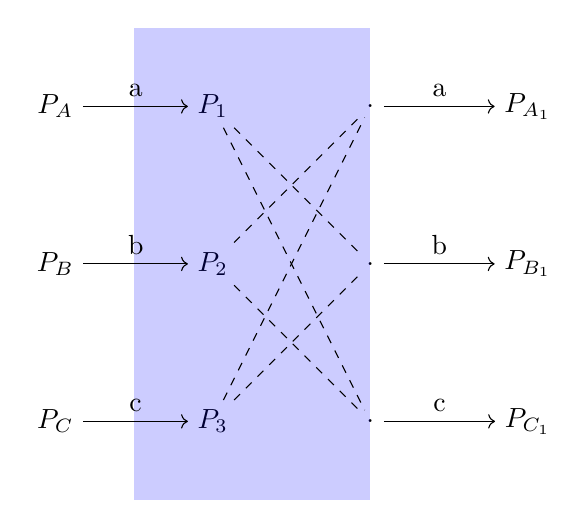
\begin{tikzpicture}
  % Nodes
  \node (A) at (0,0) {$P_A$};
  \node (B) at (0,-2) {$P_B$};
  \node (C) at (0,-4) {$P_C$};
  \node (p_a) at (2,0) {$P_1$};
  \node (p_b) at (2,-2) {$P_2$};
  \node (p_c) at (2,-4) {$P_3$};
  \node (a1) at (6,0) {$P_{A_1}$};
  \node (b1) at (6,-2) {$P_{B_1}$};
  \node (c1) at (6,-4) {$P_{C_1}$};
  \node (a) at (4,0) {$.$};
  \node (b) at (4,-2) {$.$};
  \node (c) at (4,-4) {$.$};

  % Blue rectangle
   \fill[blue, opacity=0.2] ([shift={(-1,3)}]p_b.center) rectangle ([shift={(2,-3)}]p_b.center);

  % Arrows
  \draw[->] (A) -- (p_a) node [midway,above] {a};
  \draw[->] (B) -- (p_b) node [midway,above] {b};
  \draw[->] (C) -- (p_c) node [midway,above] {c};
  \draw[dashed] (p_a) -- (b);
  \draw[dashed] (p_a) -- (c);
  \draw[dashed] (p_b) -- (a);
  \draw[dashed] (p_b) -- (c);
  \draw[dashed] (p_c) -- (a);
  \draw[dashed] (p_c) -- (b);
  \draw[->] (a) -- (a1) node [midway,above] {a};
  \draw[->] (b) -- (b1) node [midway,above] {b};
  \draw[->] (c) -- (c1) node [midway,above] {c};
\end{tikzpicture}
\end{center}
In the above figure it shows how a mixer works, as shown if three members appear and the money is paid back as shown above so that there is no link between $P_A$, $P_{A_{1}}$.
\subsection{Principles of mixing}
\begin{itemize}
    \item Use series of mixing to avoid side channel attacks, hope at least one mixer provides the anonymity.
    \item Use the same bitcoin input to the mixer because attacker can track the money taken by all users and find them, the sixe accepted by the mixer is called chunk size.
\end{itemize}
As the mixer collects its mining fee and looses the transaction fee for creating many of them so the output is less than input, if some user wants series of mixing he has to add some money which is not a good idea because anonymity is lost again.\\
So the solution for the above situation is "Fees are all or nothing", in this the mixture take everything from 1\% of number of the users of the mixer and compensates it to mixing, transaction fee, so there is 99\% chance of getting full back and 1\% chance of loosing everything.
\subsection{Continual mixing}
If a client visits a mixing service on days 1, 3, and 5, and creates three new keys before combining them to make a payment, there could be a risk of getting caught if someone has access to information about the client's visits to the mixing service, the solution for this is the clients wallet should go on mixing every day so that attacker cannot correlate those transactions.
\subsection{Decentralized mixing}
A group of themselves performs the mixing process by jumbling transactions together, enhancing privacy and anonymity using peer to peer network. They use coinjoin method to perform this.
\subsubsection{Coinjoin}
\begin{itemize}
    \item Find peers who want to perform mixing.
    \item Exchange input and output public keys.
    \item Construct the transaction and send it around themselves to sign it.
    \item Broadcast it to the miners.
\end{itemize}
While exchanging input and output address user should use multiple ip address or tor network to send them, both the input and output should not be sent at same time so anonymity is preserved.
\section{RAFT}
\subsection{Replicated state machine}
Replicated state machines are typically implemented
using a replicated log. Each server
stores a log containing a series of commands, which its
state machine executes in order. Each log contains the
same commands in the same order, so each state machine processes the same sequence of commands. Since
the state machines are deterministic, each computes the
same state and the same sequence of outputs. \\
The consensus module on a server
receives commands from clients and adds them to its log.
It communicates with the consensus modules on other
servers to ensure that every log eventually contains the
same requests in the same order, even if some servers fail.
Once commands are properly replicated, each server’s
state machine processes them in log order, and the outputs are returned to clients.
\begin{figure}[t]
\includegraphics[width=8cm]{raft rsm.png}
\centering
\caption{Replicated state machine architecture}
\end{figure}
\subsection{Consensus}
Raft implements consensus by first electing a distinguished leader, then giving the leader complete responsibility for managing the replicated log. The leader accepts
log entries from clients, replicates them on other servers,
and tells servers when it is safe to apply log entries to
their state machines.
Raft decomposes the consensus problem into two relatively independent subproblems,
\begin{itemize}
    \item \textbf{Leader election}: a new leader must be chosen when an
existing leader fails.
\item \textbf{Log replication}: the leader must accept log entries
from clients and replicate them across the cluster, forcing the other logs to agree with its own.
\end{itemize}
Raft servers communicate using remote procedure calls
(RPCs).
\subsection{Leader election}
Raft uses heartbeat to trigger leader election; servers start as followers. Followers stay in this state as long as they receive valid RPCs from a leader or candidate. Leaders send periodic heartbeats (AppendEntries RPCs with no log entries) to maintain authority. If a follower experiences an election timeout, it transitions to candidate state, increments its term, and votes for itself. The candidate issues RequestVote RPCs to other servers. The candidate remains in this state until it wins the election, another server becomes leader, or a timeout occurs.\\
To win an election, a candidate must receive votes from a majority of servers in the cluster for the same term. Each server votes for at most one candidate in a term, following a first-come-first-served basis. The majority rule guarantees only one candidate can win the election for a specific term. When a candidate wins, it becomes the leader and sends heartbeats to establish authority and prevent new elections, if no one wins there will be another election after a timeout, term is increased after every election, term is also put in messages, term also increases if no candidate was elected.
\begin{figure}[t]
\includegraphics[width=8cm]{election state.png}
\centering
\caption{Server states}
\end{figure}
\begin{figure}[t]
\includegraphics[width=8cm]{raft term.png}
\centering
\caption{Time is divided into terms}
\end{figure}
\subsection{Logs}
Each log entry stores a state machine command along with the term
number when the entry was received by the leader, log entry also has an integer index identifying its position in the log.
\begin{figure}[t]
\includegraphics[width=8cm]{raft.png}
\centering
\caption{Logs with thier composed of entries}
\end{figure}
\subsection{Logs}
\subsection{Log replication}
After being elected, the leader handles client requests by appending the command to its log as a new entry. It then replicates the entry by sending parallel AppendEntries RPCs to the other servers. Once the entry is safely replicated, the leader applies it to its state machine and returns the execution result to the client,in the event of follower crashes, slow performance, or lost network packets, the leader persists in retrying AppendEntries RPCs indefinitely until all followers successfully store all log entries. \\
A leader determines when it is safe to apply a log entry to the state machines, referred to as committed. Committed entries are guaranteed to be durable and eventually executed by all available state machines. An entry is considered committed when the leader has successfully replicated it on a majority of the servers. This commitment also applies to preceding entries in the leader's log, including those created by previous leaders.\\
If any leader fails the new leader elected should have all the committed requests from the start, so while election candidates will send their log, others should vote him if their log is subset of it. Once the new leader is elected with atleast half of votes he updates others log by sending his log. \\
To ensure coherency and safety, Raft maintains the Log Matching Property by guaranteeing that if two entries in different logs have the same index and term, they store the same command, and the logs are identical in all preceding entries. \\
During normal operation, the logs of the leader and followers remain consistent, ensuring that the AppendEntries consistency check never fails. However, leader crashes can cause inconsistencies in the logs, as the old leader may not have fully replicated all entries. These inconsistencies can accumulate over multiple leader and follower crashes, resulting in followers having missing or extra entries compared to the new leader.\\
\begin{figure}[t]
\includegraphics[width=8cm]{raft4.png}
\centering
\caption{Possible scenarios (a–f) in follower logs when a new leader comes to power: missing entries, extra uncommitted entries, or both.}
\end{figure}
To synchronize a follower's log with the leader's, the leader identifies the latest agreed-upon entry in both logs, deletes any entries in the follower's log after that point, and sends all its own entries from that point onwards to the follower. 

\subsection{Timing and availability}
Safety in Raft must not rely on timing, but availability does. Leader election is critical, and Raft requires that broadcastTime is much smaller than electionTimeout, which in turn is much smaller than MTBF. (broadcastTime $<< $electionTimeout $<<$ MTBF)
\section{Byzantine Fault Tolerance}
Since malicious attacks and software errors can cause faulty nodes to exhibit Byzantine (i.e., arbitrary) behavior, Byzantine-fault-tolerant algorithms are increasingly important.
Let us assume there are n servers and see malicious and rational 
as Byzantine rest are honest.
\subsection{consensus requirements}
\begin{itemize}
    \item \textbf{Agreement}: all honest must reach same decision.
    \item \textbf{Termination}: all honest must eventually make a decision.
    \item \textbf{Validity}: if leader is honest, no matter what all other honest ones should follow the leader.
\end{itemize}
The algorithm offers both liveness and safety
provided at most f out of a total of n replicas are simultaneously faulty. This means that clients eventually receive replies to their requests and those replies are correct according to linearizability. The algorithm works in asynchronous systems like the Internet and it
incorporates important optimizations that enable it to
perform efficiently. 
After communicating with n-f replicas twice, since f replicas might be faulty and not responding, the minimum overlap between 
them will be n-2f in the worst case f faulty replicas may be in this overlap so honest replicas are at least n-3f. so we can proove that 
$$ f <= \lfloor \frac{n -1 }{3} \rfloor$$
\section{Impossibility result}
It is impossible to have a deterministic protocol that solves consensus in a message passing asynchronous system in which at most one procees may file by crashing.
\section{PBFT}
PBFT describes a new replication algorithm that is able
to tolerate Byzantine faults.
\subsection{Quorums}
There are n = 3f + 1  nodes which are trying to achieve consensus, where f is the maximum number of byzantine nodes allowed.\\
The set of 2f + 1 or more nodes which agree on something is called a quorum.
\subsection{Properties of quorums}
\subsubsection{Intersection property}
Any two quorums have at least one honest (non byzantine) node in their intersection.\\
Let us assume A, B are two quorums and if their intersection has no non byzantine node then 
$$|A| \geq 2f + 1$$
$$|B| \geq 2f + 1$$
$$|A \cap B| \leq f$$ 
from the above 
\begin{equation}
\begin{split}
|A \cup B| & = |A| + |B| - |A \cap B| \\
 & \geq 2f + 1 + 2f + 1 - f\\
 & \geq 3f + 2\\
 & \geq n + 1
\end{split}
\end{equation}
Which is clearly a contradiction so so any two quorums has at least one honest node in intersection.
\subsubsection{Availability property}
There exists always a quorum which has no byzantine in it.
If a node hears a quorum($Q_1$) agreeing on something, then there cannot be another quorum($Q_2$) disagreeing to quorum $Q_1$, this can be proven from the intersection property. \\
if $Q_1 \cap Q_2$ contains at least one honest node, as a honest node will not contradict itself this cannot happen.
From the availability property we can guarantee liveness because byzantine nodes cannot prevent quorums from forming by being silent.
\subsection{PBFT details}
PBFT guarantees saftey because replicated service behaves as a centralized implementation that executes operations correctly one at a time, PBFT also guarantees liveness assuming week synchronous.
\begin{figure}[t]
\includegraphics[width=8cm]{pbft.png}
\centering
\caption{Normal Case Operation}
\end{figure}
\subsection{Normal Case Operation}
In the Normal Case Operation of PBFT, all correct replicas follow the three-phase protocol to achieve consensus on client requests.
The stages of PBFT and their corresponding steps:
\begin{itemize}
    \item \textbf{Request}: Client sends a request to the primary replica.
    \item \textbf{Pre-Prepare}: Primary replica assigns a sequence number to the request and multicasts a Pre-Prepare message to other replicas.
    \item \textbf{Prepare}: Replicas verify and multicast Prepare messages to vouch for the correctness of the Pre-Prepare message by observing a quorum.
    \item \textbf{Commit}: Replicas multicast Commit messages after receiving a sufficient number of valid Prepare messages, indicating the request's commitment by observing a quorum.
    \item \textbf{Reply}: Upon receiving f + 1 valid Commit messages, a replica executes the request, sends a Reply message to the client with the result, and considers the request committed.
\end{itemize}
\end{document}